\documentclass[12pt]{article}

\usepackage[margin=1in]{geometry}
\usepackage{amsmath,amsthm,amssymb,graphicx,gensymb,multicol,mathtools}
\usepackage{color}
\usepackage[english]{babel}
\usepackage[autostyle, english = american]{csquotes}
\MakeOuterQuote{"}
\graphicspath{{figures/}}
\usepackage{tikz, pgfplots}
\pgfplotsset{compat=newest}
\allowdisplaybreaks

\usepackage{biblatex}
\addbibresource{bibfile.bib}

\newcommand{\pp}{\mathbf{p}}
\newcommand{\uu}{\mathbf{u}}
\newcommand{\vv}{\mathbf{v}}
\newcommand{\ww}{\mathbf{w}}
\newcommand{\xx}{\mathbf{\hat{x}}}
\newcommand{\yy}{\mathbf{\hat{y}}}
\newcommand{\zz}{\mathbf{\hat{z}}}
\newcommand{\rr}{\mathbf{\hat{r}}}
\newcommand{\rrr}{\mathbf{r}}
\newcommand{\ppp}{\mathbf{p}}
\newcommand{\xxx}{\mathbf{x}}
\newcommand{\nnot}{\sim \!}
\let\oldemptyset\emptyset
\let\emptyset\varnothing

%for QM:
\newcommand{\intii}{\int_{-\infty}^\infty}
\newcommand{\intoi}{\int_0^\infty}
\newcommand{\HH}{\mathbb{H}}
\newcommand{\ang}[3]{\,^{#1} {#2}_{#3}}
\usepackage{braket}
\newcommand{\tr}{\mathrm{Tr}}

%units:
\newcommand{\s}{\, \mathrm{s}}
\newcommand{\m}{\, \mathrm{m}}
\newcommand{\eV}{\, \mathrm{eV}}
\newcommand{\MeV}{\, \mathrm{MeV}}
\newcommand{\ly}{\, \mathrm{ly}}

\newenvironment{problem}[2][Problem]{\begin{trivlist}
\item[\hskip \labelsep {\bfseries #1}\hskip \labelsep {\bfseries #2.}]}{\end{trivlist}}

\renewcommand{\theenumi}{\alph{enumi}}
\begin{document}

\title{Positron Converter Model}
\author{John Mastroberti}

\maketitle

\newcommand{\dxds}{\frac{dx'}{ds}}
\newcommand{\dyds}{\frac{dy'}{ds}}

\section{Background}
\label{s:background}

The positron converter provides CESR with its positrons.
The converter is a slab of heavy metal (usually tungsten), which is bombarded with electrons whose energy is on the order of $\sim 100 \MeV$.
As the incident electrons pass through the converter, they emit photons via Bremmstrahlug, which in turn decay to $e^+ e^-$ pairs:
\begin{align*}
e^- + Z \rightarrow e^- + Z + \gamma \rightarrow e^- + Z + e^+ + e^-
\end{align*}

The production of positrons in the converter is a stochastic process, the details of which are computationally expensive to simulate.
As such, it is desirable to have a model for the properties of the produced positrons (their energy, radial displacement, and direction of motion) in terms of probability distributions.

\section{Coordinate System}
\label{s:coords}

Figure 1 illustrates the coordinate system we use to describe the converter.
\begin{figure}
\centering
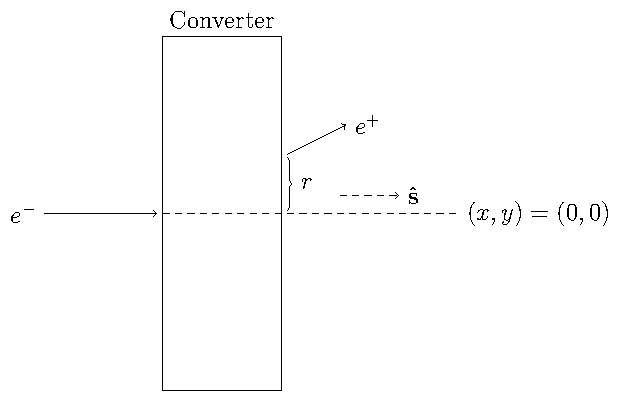
\includegraphics[width=0.6\textwidth]{coords1.pdf}
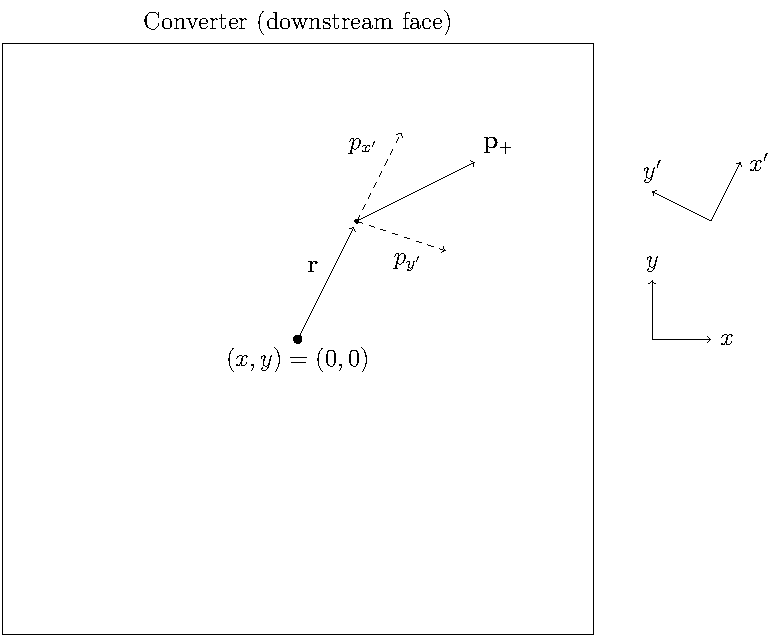
\includegraphics[width=0.8\textwidth]{coords2.pdf}
\caption{Coordinates used to describe the positrons exiting the converter.}
\end{figure}
The incoming electron beam is taken to be along the $z$-axis.
Outgoing positrons will exit the target with some displacement $r$ off of the $z$-axis, and have some energy $E_+$ and momentum $\pp_+$.
It is convenient to define a coordinate system $(x', y', z)$ with $\xx'$ pointing along the direction of $\rr$, and $\yy'$ taken perpendicular to $\xx'$ so that $(x', y', z)$ is a right-handed coordinate system.
This defines $p_x'$ and $p_y'$, the components of the outgoing positron momentum in the primed coordinate system.
We then define the "transverse momenta" $\frac{dx'}{ds}$ and $\frac{dy'}{ds}$ by
\begin{align*}
\frac{dx'}{ds} & = \frac{p_x'}{p_z} \\
\frac{dy'}{ds} & = \frac{p_y'}{p_z}
\end{align*}

\newpage

\section{The Model}
\label{s:model}

Given a positron converter of thickness $T$ and incoming electrons of energy $E_-$, we wish to predict $E_+$, $r$, $\frac{dx'}{ds}$, and $\frac{dy'}{ds}$ for the outgoing positrons.
We do this in two steps:
\begin{enumerate}
\item
First, we pull $E_+$ and $r$ from a two-dimensional probability distribution $P_1(E_+, r)$.
$P_1$ is determined by interpolation of the simulation data (see Section \ref{s:simulation}).

\item
For outgoing positrons of any given $(E_+, r)$, $\frac{dx'}{ds}$ and $\frac{dy'}{ds}$ appear to be distributed as
\begin{align*}
P_2 \left( \dxds, \dyds ; E_+, r \right) & = A \frac{1 + \beta x}{1 + \alpha_x \left( \dxds - c_x \right)^2 + \alpha_y \left( \dyds \right)^2}.
\end{align*}
Note that this functional form is empirically derived, and is not heavily motivated by the underlying physical processes that occur in the converter.
In out testing, we have found that this form does the best job of capturing the peak of the transverse momentum distribution, which is of greatest importance when the user cares about the positron capture efficiency of downstream linac elements.
For users who care more about an accurate fit to the tails of the transverse momentum distribution, a bivariate normal distribution seems to be a better fit.

\end{enumerate}



\section{Obtaining the Model Coefficients}
\label{s:simulation}

Using the Geant4\cite{geant} software package developed at CERN, we have developed a program for simulating the production of positrons in the converter.
This program simulates the results of sending electrons of a fixed energy into a target of fixed thickness, and records the $E_+$, $r$, $\dxds$, and $\dyds$ values of the positrons that emerge at the downstream face of the converter.
The number of electrons used is determined dynamically so that good statistics on the properties of the produced positrons can be obtained.

With a large sample of positron data in hand, the program first bins the $E_+$ and $r$ data into a 2D histogram.
This binned data can then be interpolated to approximate the distribution of $E_+$ and $r$ values, $P_1(E_+, r)$.
After the $(E_+, r)$ bins are chosen, the $\dxds$ and $\dyds$ values for positrons in each bin are then themselves binned into 2D histograms.
We then fit the functional form described in Section \ref{s:model} to the binned $\dxds$, $\dyds$ data in each of the $(E_+, r)$ bins to obtain the fit parameters $A$, $\beta$, $\alpha_x$, $\alpha_y$ and $c_x$.
These fits gives us an approximation of $P_2 \left( \dxds, \dyds ; E_+, r \right)$.

Note that the distributions $P_1$ and $P_2$ will vary with incoming electron energy $E_-$ and target thickness $T$.
The program can be used to sample the behavior of the converter at various values of $E_-$ and $T$, and performs the above procedure once per $(E_-, T)$ pair.
\textit{Bmad} will then interpolate between the discrete set of $(E_-, T)$ values simulated to model the converter at any electron energy and target thickness in the range of interest.



\printbibliography


\end{document}
